% MAS1004 Assignment 1: long report.
%
% You fill this in with your agent, in your repository. AGENTS.md tells the
% agent how. Red text in the PDF is what still has to be replaced.
%
% - Pictures go in figures/. Copy them from results/, which is not in git.
% - Outputs go in outputs/. run.py saves what it prints in
%   results/<tag>_output.txt, and PLAN.md saves the other outputs in results/
%   with `| tee results/...`. Copy them here. \outputfile{outputs/check.txt}
%   prints a file exactly as it is. Every number in this report has to come
%   from such an output.
%
% To make the PDF: compress this folder into a zip, and on Overleaf choose
% New Project, Upload Project. Set Menu, Compiler to XeLaTeX, and Recompile.
\documentclass[11pt]{article}
\usepackage[ko]{mas1004}

\reporttitle{assignment1: Long Report}
\studentname{}
\studentid{}

\begin{document}
\makeheader

% ---------------------------------------------------------------------------
\section*{Problem 1. 카테고리와 이미지}

\subsection*{카테고리를 고른 이유}
저는 캐릭터라는 주제를 골랐고, 카테고리로는 치이카와, 농담곰, 듀 가나디,
몰랑이 네 가지를 정했습니다. 이 캐릭터들은 요즘 중고등학생부터 대학생까지
많은 사람들이 좋아하는 캐릭터이고, 저 역시 평소에 관심을 가지고 있던
캐릭터들이라 자연스럽게 이 주제를 고르게 되었습니다.

이 네 캐릭터를 고른 데에는 생김새가 서로 많이 닮았다는 이유도 있습니다.
넷 모두 흰 몸에 눈, 코, 입과 몸의 윤곽이 검은 선으로 그려져 있고, 그중
치이카와, 농담곰, 몰랑이는 작은 귀까지 비슷합니다. 특히 치이카와와
농담곰은 같은 작가의 캐릭터라 그림체도 거의 같습니다. 사람은 이 캐릭터들을
어렵지 않게 구분하지만, 막상 무엇을 보고 구분하는지 설명하려고 하면
생각보다 미묘한 차이라는 것을 느꼈습니다. 그래서 모델도 이 미묘한 차이를
찾아낼 수 있을지 궁금했습니다. 또한 ResNet18은 실제 사진으로 학습된
모델인데, 단순한 선과 면으로 이루어진 캐릭터 그림에서도 그 지식을 활용할
수 있을지도 알고 싶었습니다.

\subsection*{모델이 사용할 것이라고 예상한 특징}
학습 전에는 모델이 각 캐릭터의 생김새, 그중에서도 특징이 되는 부분을 보고
구분할 것이라고 예상했습니다. 치이카와는 다른 캐릭터들보다 눈이 크고 모양이
달라서 눈으로, 듀 가나디는 다른 캐릭터보다 조금 더 큰 귀로, 몰랑이는 몸의
형태가 나머지와 많이 달라서 몸의 생김새로 구분할 것이라고 생각했습니다.
농담곰은 듀 가나디와 비슷한 점이 많아서 무엇으로 구분할지 예상하기
어려웠습니다. 만약 모델이 제 예상처럼 생김새로 구분하지 않는다면, 그 대신
무엇을 보고 판단하는지 알아내는 것이 이번 과제에서 가장 알고 싶은 점이었습니다.

\subsection*{이미지 수}
검색어는 chiikawa에는 ``chiikawa'', nongdamgom에는 ``自分ツッコミくま'',
ganadi에는 ``듀 가나디'', molang에는 ``molang 몰랑이''를 사용했다.
첫 학습 출력에 따르면 각 클래스에서 150장씩, 총 600장을 받았다.

\begin{center}\footnotesize
\begin{tabular}{lr}
	oprule
클래스 & 다운로드 이미지 \\
\midrule
chiikawa & 150 \\
ganadi & 150 \\
molang & 150 \\
nongdamgom & 150 \\
\bottomrule
\end{tabular}
\end{center}

% ---------------------------------------------------------------------------
\section*{Problem 2. 이미지 전처리}

\picturefile[0.95\linewidth]{figures/problem2_chiikawa_crop.jpg}

그림은 치이카와 단체샷이다. 원본의 가운데 정사각형을 224×224로 자르면
가장자리 캐릭터가 잘려 나가고, 그림에서 중요한 치이카와도 크롭 안에서
잘려 나간다. 위 그림의 오른쪽은 실제로 모델이 보는 가운데 크롭이다.
전처리는 짧은 변을 256으로 bilinear resize한 다음 중앙 224×224를 자르고,
RGB 채널을 ImageNet 평균과 표준편차로 정규화했다.

% ---------------------------------------------------------------------------
\section*{Problem 3. 첫 학습 결과}

\begin{center}\footnotesize
\resizebox{\linewidth}{!}{%
\begin{tabular}{lllr rrrr}
\toprule
tag & start & trained & epochs & lr & trainable parameters & train accuracy & test accuracy \\
\midrule
run & ImageNet & 전체 & 10 & 0.0001 & 11,178,564 & 100.0\% & 97.5\% \\
scratch & random & 전체 & 10 & 0.0001 & 11,178,564 & 100.0\% & 63.3\% \\
frozen & ImageNet & 마지막 층 & 10 & 0.001 & 2,052 & 95.0\% & 92.5\% \\
custom & ImageNet & 전체 & 5 & 0.0003 & 11,178,564 & 100.0\% & 97.5\% \\
\bottomrule
\end{tabular}
}
\end{center}

\begin{center}
\picturefile[0.48\linewidth]{figures/run_curves.png}\hfill
\picturefile[0.48\linewidth]{figures/run_confusion.png}
\end{center}
\begin{center}
\picturefile[0.48\linewidth]{figures/scratch_curves.png}\hfill
\picturefile[0.48\linewidth]{figures/scratch_confusion.png}
\end{center}
\begin{center}
\picturefile[0.48\linewidth]{figures/frozen_curves.png}\hfill
\picturefile[0.48\linewidth]{figures/frozen_confusion.png}
\end{center}
\begin{center}
\picturefile[0.48\linewidth]{figures/custom_curves.png}\hfill
\picturefile[0.48\linewidth]{figures/custom_confusion.png}
\end{center}

run의 train loss는 첫 epoch의 0.7575에서 2번째 epoch에 0.1283으로 크게
내려갔고 이후 0에 가까워졌다. test loss는 4번째 epoch에 0.1117까지
내려온 뒤 대체로 0.10 근처에서 평평해졌다. test 정확도도 4번째 epoch의
97.5\% 부근 이후 더 오르지 않았다. 학습은 초반에 대부분 진행됐고,
뒤쪽 epoch은 train 성능만 더 완벽하게 만들었다.

run의 train/test 정확도 차이는 \textbf{직접 계산}하면
$100.0-97.5=2.5$퍼센트포인트다. scratch는 $100.0-63.3=36.7$퍼센트포인트다.
run은 검색 이미지의 test를 거의 맞혔지만, 새 이미지에서의 성능은 별도로
확인해야 했다. scratch는 train을 외우는 데 비해 test 일반화가 약했다.

run confusion matrix에서 오답은 치이카와→가나디 1장, 치이카와→몰랑이 1장,
농담곰→몰랑이 1장으로 각기 다른 조합이었다. 반복되는 최다 혼동 쌍은
없었다. 같은 작가의 치이카와와 농담곰이 가장 헷갈릴 것이라는 예상과 달리
둘 사이 오답은 없었다.

ImageNet 시작과 random 시작의 test 정확도 차이는 \textbf{직접 계산}하면
$97.5-63.3=34.2$퍼센트포인트다. ImageNet이 선·윤곽·둥근 형태 같은 특징을
이미 학습해 캐릭터 그림에 활용했을 가능성이 있다고 생각한다. 마지막 층만
학습한 frozen의 test 정확도는 92.5\%로, 전체 학습 run보다
	extbf{직접 계산} 기준 5.0퍼센트포인트 낮았다. frozen은 2,052개,
전체 학습 run은 11,178,564개 파라미터를 학습했다.

\subsection*{실행 출력}
\outputfile{outputs/run_output.txt}
\outputfile{outputs/scratch_output.txt}
\outputfile{outputs/frozen_output.txt}
\outputfile{outputs/custom_output.txt}

% ---------------------------------------------------------------------------
\section*{Problem 4. 데이터 청소와 재학습}

\subsection*{청소 규칙}
\paragraph{청소를 시작하기 전에 쓴 규칙}
모델이 캐릭터의 생김새만 보고 구분하고, 그 생김새로 그림뿐 아니라 굿즈
같은 다른 형태에서도 알아보기를 원했다. 그래서 한 캐릭터가 화면의 주인공이면
형태와 상관없이 남기되, 캐릭터 이름 글자가 보이는 이미지는 그림이든 굿즈든
뺐다. 처음에는 다른 캐릭터가 같은 비중으로 함께 나오는 단체샷도 제외하기로 했다.

\paragraph{이미지를 보다가 바꾼 규칙: 단체샷 기준}
같은 비중인 단체샷이 너무 많아 모두 빼면 데이터가 크게 줄 것 같아 기준을
바꿨다. 224×224 크롭 미리보기를 기준으로, 크롭 안에서 대상 캐릭터가 잘려
나가거나 다른 캐릭터가 더 크게 보이면 뺐다. 대상 캐릭터가 크롭 안의 주인공이면
단체샷이어도 남겼다. prepare\_image는 가운데 정사각형만 남기므로, 크롭 안의
캐릭터가 모델이 실제로 보는 대상이라고 판단했다. 크롭 가장자리에 다른 캐릭터
일부가 보일 수 있다는 점은 감수했다.

그 밖에는 캐릭터 이름 글자가 읽힐 정도로 보이는 이미지, 해당 캐릭터가 없거나
글자가 대부분인 이미지를 뺐다. 갈색 몰랑이는 현재 흰 몰랑이 카테고리에
포함되지 않는다고 보아 제외했다. 캐릭터가 너무 작아 224×224에서 알아보기
어려운 이미지도 제외했고, 특징이 살아 있는 다른 그림체의 팬아트는 남겼다.
거의 같은 이미지는 한 장만 남기고 나머지를 뺐다.

\subsection*{찾은 불필요 이미지 유형}
세 예시는 모두 삭제한 원본에서 가져왔다.

\begin{center}\small
\begin{minipage}{0.31\linewidth}\centering

\includegraphics[width=\linewidth]{figures/junk_other_character_chiikawa_0004.jpg}\\
chiikawa/0004.jpg — 다른 캐릭터
\end{minipage}\hfill
\begin{minipage}{0.31\linewidth}\centering

\includegraphics[width=\linewidth]{figures/junk_name_text_molang_0001.jpg}\\
molang/0001.jpg — 이름 글자
\end{minipage}\hfill
\begin{minipage}{0.31\linewidth}\centering
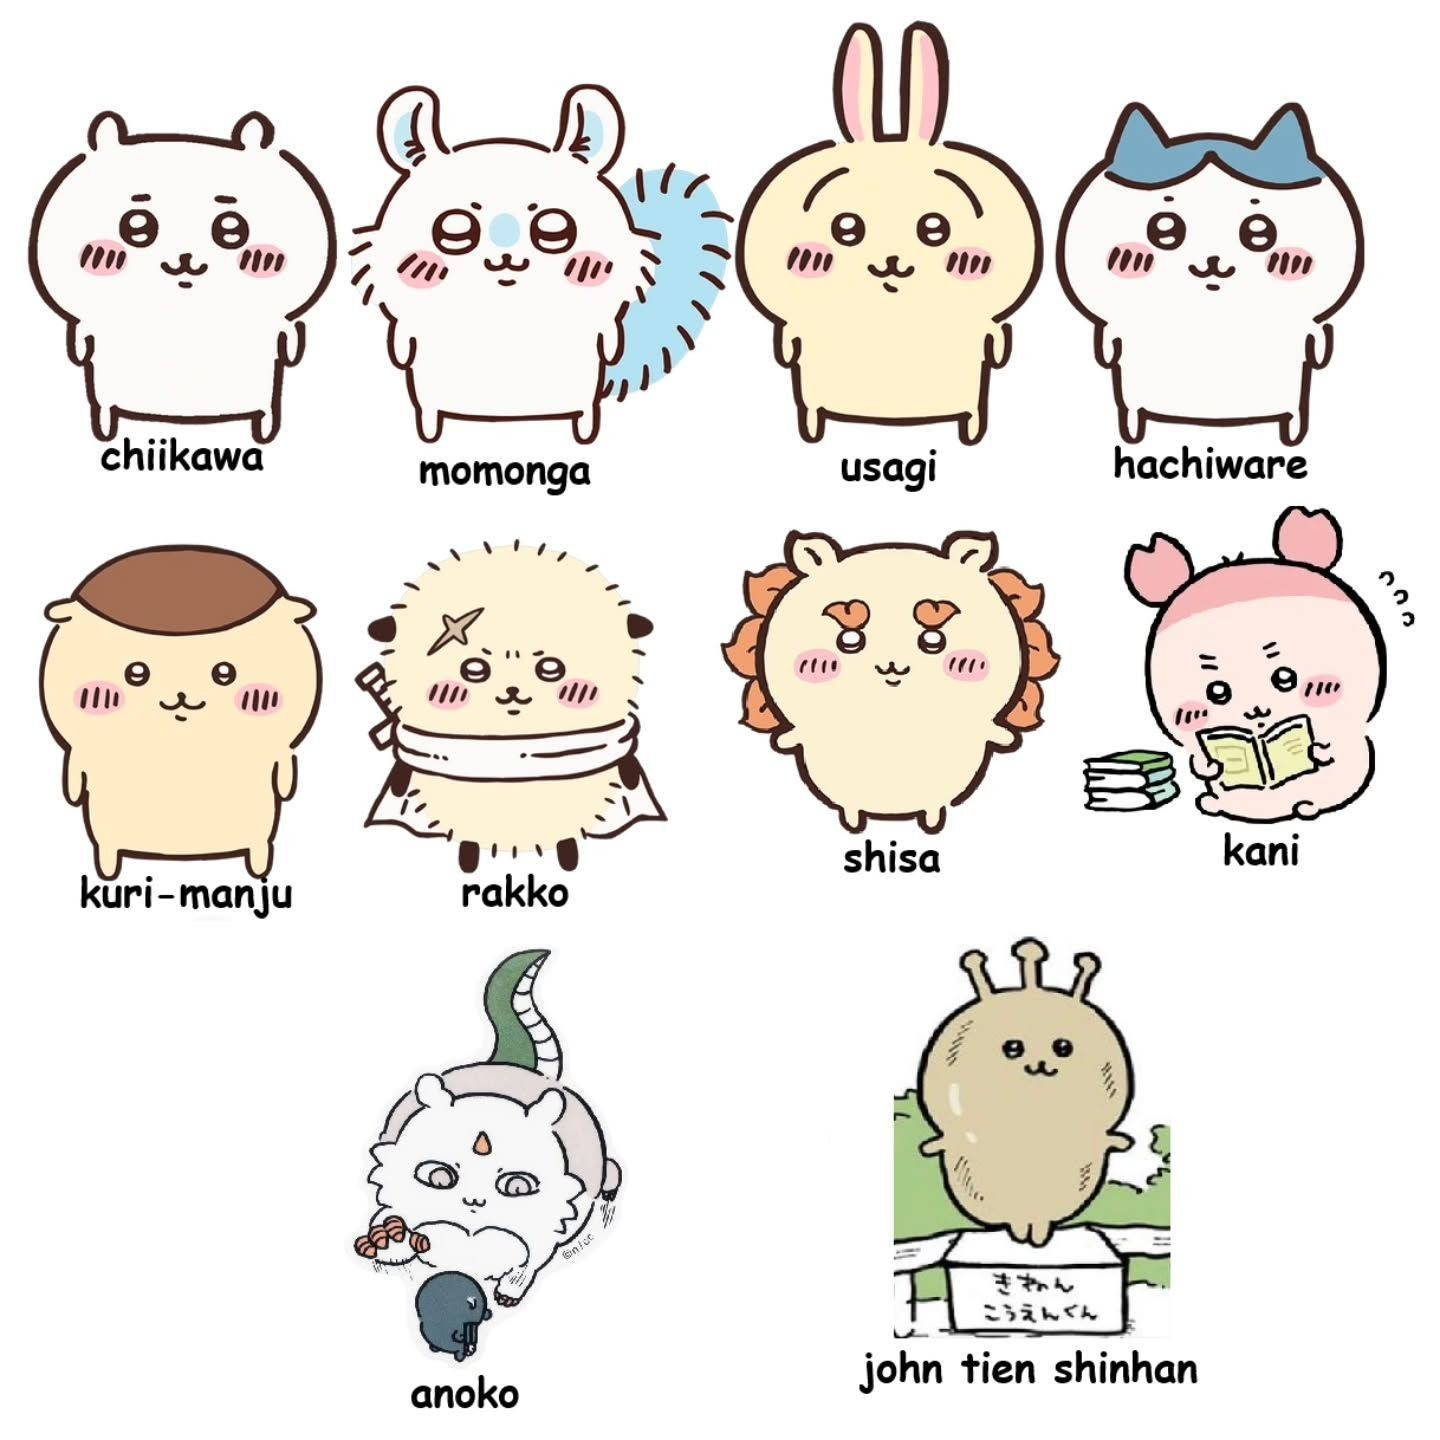
\includegraphics[width=\linewidth]{figures/junk_group_shot_chiikawa_0001.jpg}\\
chiikawa/0001.jpg — 단체샷
\end{minipage}
\end{center}

\subsection*{제거 수와 near copy}
\outputfile{outputs/clean_count.txt}
\outputfile{outputs/clean_reason_by_class.txt}

공식 clean.py count 기준 제거 수는 chiikawa 84장, ganadi 42장, molang
72장, nongdamgom 25장이다. 네 클래스 제거 수 합계 223장과 전체 600장 중
377장이 남았다는 값은 표의 클래스를 더한 \textbf{직접 계산}이다.
가장 많은 제거 이유는 name text 102장이었다.

청소 전 data/raw 복사본으로 재현한 공식 suspects agreement는 600장 중
83.0\%였고, 기존 메모와 일치했다. 당시 공식 copies.png 제목은 near copy
44쌍을 표시했다. 현재 청소 결과로 공식 copies 시트에는 9쌍이 표시된다.
clean.py count에서 near copy 이유로 24장을 제거한 것으로 출력됐다.
세 장이 한 묶음이었던 ganadi/0041, 0080, 0112에서는 0041만 남겼다.
chiikawa/0012와 0023은 서로 중복으로 보였지만 이름 글자 규칙에도 걸려
둘 다 뺐다. 일부는 양쪽을 남겨두었다.

확인하지 못해 둘 다 남겨둔 쌍은 nongdamgom/0027과 0130,
nongdamgom/0013과 0058, ganadi/0110과 0136, ganadi/0062와 0102이다.
ganadi/0062와 0102에는 ``듀…'' 글자가 있었다. copies.png에서 화면에
표시되지 않았던 다섯 쌍도 확인하지 못해 보류했다.

\begin{center}
\picturefile[0.9\linewidth]{figures/preclean_near_copies.png}
\picturefile[0.9\linewidth]{figures/cleaned_near_copies.png}
\end{center}
\outputfile{outputs/suspects_preclean_output.txt}
\outputfile{outputs/suspects_top20_removed.txt}

\begin{center}\small
\begin{tabular}{lrr}
\toprule
클래스 & 공식 상위 20개 중 제거 & 그중 학습 후 too small \\
\midrule
chiikawa & 12/20 & 0 \\
ganadi & 11/20 & 1 (0086, 1위) \\
molang & 7/20 & 1 (0079, 2위) \\
nongdamgom & 4/20 & 0 \\
\bottomrule
\end{tabular}
\end{center}

suspects는 놓친 불량을 포함했다. ganadi/0086과 molang/0079를 처음에는
남겼다가 clean 모델의 오분류를 다시 보고 too small 사유로 제거했다.
반대로 도구 상위 20개에 들지 않은 제거 파일도 많았다. 상위 20개 제거 수
합계 34장은 위 표에서 직접 합산한 값이다. 이름 글자 이미지처럼 규칙으로
찾은 불량은 suspects 상위권에서 놓친 경우가 있었다.

\subsection*{청소 전후}
\outputfile{outputs/compare.txt}

최종 비교에서 run의 검색 test 정확도는 97.5\%, clean은 92.1\%로 청소 후 오히려 낮아졌다.
나는 이것이 모델이 나빠졌다기보다 시험이 더 정직해졌기 때문이라고 생각한다.
청소로 뺀 223장 중 가장 많은 것은 캐릭터 이름 글자가 보이는 이미지(102장)와
거의 같은 이미지(24장)였다. 이름이 적혀 있으면 생김새를 몰라도 글자로 답을 알 수 있고,
같은 그림이 train과 test에 나뉘어 있으면 외운 것을 그대로 맞히면 된다.
청소 전 97.5\%에는 이런 쉬운 문제가 섞여 있었을 가능성이 높다.

또 청소 전후의 test 집합은 같은 시험지가 아니다. 청소 전 test는 120장이었고
청소 후에는 76장이라, 한 장 틀릴 때마다 움직이는 정확도가 더 크다.
그래서 test 정확도만으로는 청소의 효과를 판단하기 어렵다고 보고,
청소와 상관없이 바뀌지 않는 새 이미지 32장으로 다시 비교했다.

새 이미지에서는 run이 46.9\%(15/32), clean이 53.1\%(17/32)로 청소 후 모델이 더 잘 맞혔다.
test 정확도는 떨어졌지만 처음 보는 이미지는 더 잘 맞혔다는 점에서,
청소가 모델을 쉬운 단서 대신 실제 생김새 쪽으로 조금 더 기울게 했다고 생각한다.
다만 차이가 32장 중 2장뿐이라 이것만으로 청소 효과를 확신하기는 어렵다.
(53.1 $-$ 46.9 = 6.2퍼센트포인트는 출력값에서 직접 계산한 값이다.)

최종 청소 모델의 혼동 행렬과 자신 있게 틀린 이미지 6장은 다음과 같다.
\begin{center}\picturefile[0.48\linewidth]{figures/clean_confusion.png}\hfill
\picturefile[0.48\linewidth]{figures/clean_worst.png}\end{center}

% ---------------------------------------------------------------------------
\section*{Problem 5. 새로운 출처의 이미지}

새 이미지는 직접 그린 그림과 직접 촬영한 굿즈 사진으로 준비했다.
다운로드 이미지 검색과 겹칠 수 없는 개인 그림·사진이다.
공식 overlap 출력은 이 이미지들이 다운로드한 599장과 near copy가 아니라고
보고했다.

\outputfile{outputs/overlap.txt}

최종 clean 모델은 다운로드 test에서 92.1\%, 새 이미지에서 53.1\%였다.
청소 전 run은 각각 97.5\%, 46.9\%였다. 새 이미지의 배경, 조명, 재질과
촬영 각도가 검색 이미지와 달라 결과가 낮아졌을 수 있다.

\subsection*{자신 있게 틀린 다섯 이미지}
\picturefile[0.95\linewidth]{figures/new_images_confident_mistakes.png}

1. 농담곰 굿즈를 가나디로 98\% 예측했다. 얼굴만 보이는 네모 파우치라
    귀와 몸통이 드러나지 않고 비닐 반사도 있다. 네모 파우치 모양을
    가나디로 읽었을 수도 있다고 생각한다.
2. 치이카와 연필 그림을 가나디로 97\% 예측했다. 회색 선만 있어서
    검은 선화가 많은 가나디로 답했을 수도 있다고 생각한다.
3. 치이카와 보라색 선 그림을 몰랑이로 95\% 예측했다. 보라색과 배경이
    몰랑이 이미지의 다양한 색을 떠올리게 했을지 모르겠지만 확실하지 않다.
4. 농담곰 스티커 시트를 몰랑이로 83\% 예측했다. 작은 캐릭터, 파스텔
    배경, 비닐 포장 또는 한 화면에 많은 캐릭터가 영향을 줬을 수 있다.
5. 몰랑이 굿즈를 가나디로 80\% 예측했다. 보라·파란 조명 아래 몰랑이가
    작게 보여서 틀렸을 수 있다고 생각한다.

새 이미지에는 책상과 다른 굿즈 같은 배경, 색이 낀 조명과 비닐 반사,
얼굴 클로즈업과 누운 자세, 천·스티커·연필선 같은 재질 차이가 있었다.

% ---------------------------------------------------------------------------
\section*{Problem 6. 데모 페이지}

주소: \url{https://slowwbluee.github.io/mas1004_assignment_01/}

상위 배지는 로컬과 배포 페이지에서 초록색이었다. 카테고리에 없는 장난감
피규어 여러 개 사진을 보여줘도 모델은 ``해당 없음'' 대신 네 캐릭터 중
하나를 골라 답했다. 따라서 높은 확신도가 정답을 뜻하지 않는다.

% ---------------------------------------------------------------------------
\section*{Problem 7. 모델이 무엇을 보는가}

Problem 1에서는 눈·귀·몸 모양을 단서로 구분할 것이라고 예상했다. 아래 세
가설은 이미지와 오답에서 발견한 단서를 바탕으로 세웠고, 지정한 부분만
바꾼 원본/사본을 데모 페이지에 각각 올려 확인했다.

\subsection*{가설 1: 농담곰 굿즈의 배경이 노란색이면 농담곰으로 인식한다}
노란 배경의 농담곰 굿즈는 농담곰으로 답했고, 민트·검은 배경의 비슷한
굿즈는 가나디로 답한 점에서 배경 색을 의심했다. 노란 배경 치이카와
키링은 치이카와로 맞혔으므로, 가설 범위를 농담곰 굿즈로 한정했다.
같은 굿즈의 캐릭터 부분을 유지하고 배경을 노란색으로 바꾸는 실험은
배경 단서가 답에 영향을 주는지 확인하기 위한 것이었다.

\begin{center}
\begin{tabular}{llll}
\toprule
번호 & 원본 & 노란 배경 사본 & 농담곰 확률 \\
\midrule
23 & 가나디 52.7\% & 농담곰 74.7\% & 5.5\% $\rightarrow$ 74.7\% \\
25 & 가나디 31.5\% & 농담곰 88.4\% & 23.3\% $\rightarrow$ 88.4\% \\
27 & 가나디 34.4\% & 농담곰 57.8\% & 7.5\% $\rightarrow$ 57.8\% \\
30 & 가나디 94.6\% & 농담곰 50.4\% & 4.4\% $\rightarrow$ 50.4\% \\
\bottomrule
\end{tabular}
\end{center}

실험 1 네 장 모두 원본에서는 가나디가 1등이었고, 노란 배경 사본에서는
농담곰이 1등이었다. 다만 칠하는 과정에서 포장 비닐과 주변 물건도 함께
사라졌으므로, 노란색과 배경 단순화 효과를 분리하지 못했다. 30번 사본은
농담곰 50.4\%, 가나디 47.5\%로 차이가 작았다.
실험 1 사본은 에이전트가 배경을 제대로 분리하지 못해 내가 직접 색칠해서 만들었다.

\subsection*{가설 2: 색깔 선 그림은 몰랑이로 분류된다}
색깔 펜으로 그린 다른 캐릭터들도 몰랑이로 분류된 사례가 있었고,
보라색 선 치이카와와 색깔 선 가나디도 그랬다. 반면 회색 연필 그림의 답은
흩어졌다. 흰 종이 배경은 비슷했으므로 선 색이 단서일 수
있다고 생각했다. 선의 굵기와 위치를 유지하고 색만 검정으로 바꿔 이를
시험했다(실험 2).

\textbf{사본 방향 문제와 수정.} 처음 받은 실험 2, 3의 사본은 에이전트가
변형하는 과정에서 사진의 회전 정보(EXIF)를 빠뜨려, 원본과 90도 다른 방향으로
저장되어 있었다. 그러면 색뿐 아니라 방향도 같이 바뀐 것이라 변형이 가설을
제대로 시험하지 못한다. 비교 시트에서 이 문제를 발견하고, 사본의 방향을
원본과 같게 맞춘 뒤 데모 페이지에 직접 다시 올려 결과를 확인했다.
아래 실험 2, 3의 표는 방향을 고친 뒤의 결과이다. 실험 3의 20번은 처음부터
방향이 맞아 기존 결과를 그대로 썼다.

\begin{center}
\begin{tabular}{llll}
\toprule
번호 & 원본 & 검정 선 사본 & 몰랑이 확률 \\
\midrule
09 (치이카와) & 몰랑이 94.4\% & 가나디 53.1\% & 94.4\% $\rightarrow$ 25.4\% \\
11 (가나디) & 몰랑이 47.3\% & 가나디 99.3\% & 47.3\% $\rightarrow$ 0.5\% \\
12 (가나디) & 몰랑이 92.6\% & 가나디 74.7\% & 92.6\% $\rightarrow$ 20.1\% \\
13 (가나디) & 몰랑이 94.3\% & 가나디 97.9\% & 94.3\% $\rightarrow$ 1.6\% \\
\bottomrule
\end{tabular}
\end{center}

네 장 모두 선 색만 검정으로 바꾸자 몰랑이에서 가나디로 답이 바뀌었다.
가나디 그림 세 장은 정답을 맞히게 되었고, 치이카와 그림도 몰랑이가 아닌
가나디가 되었다. 방향을 고치기 전에는 보라색 선 치이카와가 검정으로 바꾼
뒤에도 몰랑이로 남는 예외였는데, 방향을 맞추자 예외가 사라져 가설 2를 더
강하게 뒷받침했다. 바뀐 답이 모두 가나디였다는 점은 ``검정 선이면
가나디''라는 추측도 지지한다. 다만 색깔 펜과 연필은 선 굵기·진하기도 달라서,
이 실험은 굵기를 그대로 두고 색만 바꿔 그 차이를 줄이려 했다.

\subsection*{가설 3: 모델은 몰랑이를 색으로 알아본다}
색이 있는 다른 캐릭터와 피규어 사진이 몰랑이로 분류된 사례가 있었고,
몰랑이 학습 이미지의 배경 색도 다양했다. 색이 몰랑이 답에 쓰인다면
몰랑이 사진을 흑백으로 바꿨을 때 답이 달라질 것이라고 예상했다(실험 3).

\begin{center}
\begin{tabular}{llll}
\toprule
번호 & 원본 & 흑백 사본 & 몰랑이 확률 \\
\midrule
17 & 몰랑이 93.2\% & 가나디 57.6\% & 93.2\% $\rightarrow$ 6.5\% \\
18 & 몰랑이 97.4\% & 몰랑이 53.5\% & 97.4\% $\rightarrow$ 53.5\% \\
19 & 몰랑이 93.4\% & 가나디 36.0\% & 93.4\% $\rightarrow$ 27.9\% \\
20 & 몰랑이 52.3\% & 농담곰 52.8\% & 52.3\% $\rightarrow$ 7.2\% \\
\bottomrule
\end{tabular}
\end{center}

네 장 모두 몰랑이 확률이 크게 떨어졌고, 그중 세 장은 몰랑이가 아닌 다른
캐릭터가 되었다. 하지만 18번은 흑백이어도 몰랑이가 1등으로 남았다.
방향을 고치기 전에는 네 장 모두 몰랑이가 아니게 되었는데, 방향을 맞추자
효과가 줄었다. 처음 결과는 흑백과 회전이 함께 작용해 부풀려졌던 것이고,
회전 자체도 모델의 답에 영향을 준다는 뜻이다. 따라서 색이 몰랑이 판단에
큰 영향을 주는 것은 맞지만, 색만 없애면 몰랑이를 전혀 알아보지 못한다고까지
말하기는 어렵다. 반대 사례로 회색 연필로 그린 몰랑이도 색이 없어도
몰랑이로 맞혔지만, 확신도는 낮았다.

\subsection*{세 실험을 함께 보며}
색을 빼면 가나디로 가는 경향은 실험 2와 실험 3에서 함께 보였다.
색깔 펜 선을 검정으로 바꾼 그림 네 장이 모두 가나디가 되었고, 흑백으로
바꾼 몰랑이 사진 중 두 장도 가나디로 분류됐다. Draw it 그림이 모두
가나디로 나온 기록과도 비슷하다. 반대로 색이 있으면 몰랑이로 가는 경향은
실험 2 원본과 실험 3 원본에서 보였다. Problem 1에서는 눈, 귀, 몸 모양으로
구분할 것이라고 예상했다.

\subsection*{에이전트에게 보낸 이미지 변형 요청 원문}
(요청문의 ``실험 2-A''는 본문의 실험 2를 가리킨다.)
\begin{quote}\small
{\bfseries [요청 1: 이미지 변형]}\\
Problem 7 실험용 이미지 변형을 부탁할게. 아까 번호를 붙인 새 이미지 기준이야.\\
세 가지 모두 원본은 절대 건드리지 말고 사본만 만들어줘.\\
각 실험마다 번호별 실제 파일명도 같이 알려줘.\\[0.4em]
{\bfseries [실험 1] 23, 25, 27, 30번 (농담곰 굿즈)}\\
배경만 노란색으로 바꾼 사본을 data/changed/exp1\_background\_yellow 에 저장해줘.\\
굿즈 자체의 색, 모양, 위치, 크기는 그대로 두고 배경만 바꿔줘.\\[0.4em]
{\bfseries [실험 2-A] 09, 11, 12, 13번 (색깔 펜 그림)}\\
선 색만 검정으로 바꾼 사본을 data/changed/exp2a\_lines\_black 에 저장해줘.\\
선의 굵기, 위치, 모양과 종이 배경은 그대로 두고 선 색만 바꿔줘.\\[0.4em]
{\bfseries [실험 3] 17, 18, 19, 20번 (몰랑이 사진)}\\
흑백으로 바꾼 사본을 data/changed/exp3\_molang\_gray 에 저장해줘.\\
색만 없애고 크기, 위치, 밝기는 최대한 그대로 둬줘.\\[0.4em]
다 만들면 실험별로 원본과 사본을 나란히 보여주는 비교 시트도 만들어줘.\\
예측이나 결과 판단은 하지 마. 이미지 변형만 해줘.\\[0.6em]
{\bfseries [요청 2: 실험 1 다시 요청]}\\
실험 1 사본이 내가 원한 대로 안 됐어. 노란색이 거의 안 보여.\\
23, 25, 27, 30번 각각 농담곰 캐릭터 그림이나 인형 부분만 그대로 두고,\\
그 외의 영역은 포장 종이, 비닐, 주변 물건까지 전부 노란색으로 바꿔줘.\\
특히 원래 민트색, 검은색이던 부분은 반드시 노랗게 바뀌어야 해.\\
캐릭터 자체의 색, 모양, 위치, 크기는 바꾸지 마.\\
data/changed/exp1\_background\_yellow의 사본을 다시 만들고\\
비교 시트도 새로 만들어줘. 원본은 건드리지 마.\\
예측이나 결과 판단은 하지 마.\\[0.6em]
{\bfseries [요청 3: 실험 1 중단]}\\
실험 1 배경 작업은 중단해. 내가 직접 칠한 사본을 쓸 거야.\\
data/changed/exp1\_background\_yellow\_manual 폴더에 있는 이미지를 실험 1 사본으로 써줘.\\
이 폴더 파일은 절대 수정하거나 덮어쓰지 마.\\
→ 이후 실험 1 사본은 내가 직접 칠해서 만들었음.
\end{quote}
에이전트가 만든 실험 2, 3 사본은 방향이 틀어져 있어, 위에 적은 대로 사본의
방향은 내가 직접 원본과 같게 맞췄다.

실험별로 모델 입력과 같은 224×224 크롭을 나란히 비교했다. 실험 2, 3 비교
그림은 방향을 고치기 전의 사본으로 만든 것이라 사본이 원본과 90도 돌아가
있다(그림 제목의 ``2-A''는 실험 2를 가리킨다). 이 그림에서 방향 문제를
발견했다.
\begin{center}\picturefile[0.95\linewidth]{figures/problem7_exp1_crops.png}\end{center}
\begin{center}\picturefile[0.95\linewidth]{figures/problem7_exp2_crops.png}\end{center}
\begin{center}\picturefile[0.95\linewidth]{figures/problem7_exp3_crops.png}\end{center}

아래 출력은 에이전트가 데모 페이지에서 읽은 결과이다. 실험 1은 최종 결과와
같고, 실험 2, 3 사본 값은 방향을 고치기 전의 값이다. 방향을 고친 뒤의 값은
내가 데모 페이지에 직접 올려 확인했고 위 표에 적었다.
\outputfile{outputs/problem7_demo_results.txt}

\subsection*{현재 생각과 확신}
지금 모델은 무엇으로 캐릭터를 구분한다고 생각하나: Problem 1에서는 눈,
귀, 몸 모양 같은 생김새로 구분할 거라고 예상했다. 하지만 실험 결과를
보면 모델은 생김새보다 색에 크게 기대어 구분하는 것 같다. 그림 선에 색이
있거나 사진에 색이 많으면 몰랑이로, 색이 없으면 가나디로, 농담곰 굿즈는
노란 배경이면 농담곰으로 답하는 경향이 있었다.

얼마나 확신하나, 그 이유: 60\% 정도 확신한다. 캐릭터 모양은 그대로 두고
색만 바꿨는데 답이 바뀌었다. 색깔 선을 검정으로 바꾸자 네 장 모두
몰랑이에서 가나디가 됐고, 몰랑이를 흑백으로 바꾸자 네 장 모두 몰랑이
확률이 크게 떨어졌고, 농담곰 굿즈의 배경을 노랗게 바꾸자 네 장 모두
농담곰이 됐다. 세 실험 모두 색만 건드렸는데 답이 움직였다.

다만 100\%라고 하기 어려운 이유도 있다. 실험마다 이미지가 4장뿐이고,
실험 1은 배경을 칠하면서 비닐과 주변 물건도 같이 사라져 노란색 때문인지
배경이 단순해져서인지 구분할 수 없다. 흑백 몰랑이 중 한 장은 여전히
몰랑이로 분류되었고, 회색 연필로 그린 몰랑이도 색이 없는데 몰랑이로
맞혔다. 또 사본 방향을 고치기 전후로 결과가 달라진 것을 보면, 색 외에
방향 같은 다른 요인도 모델의 답에 영향을 준다.

아직 확인하지 못한 것과 새 추측: 색으로 분류하는 특징이 모든 캐릭터에도
적용되는지는 모르겠다. 치이카와 그림은 선 색을 바꾸자 답이 바뀌었지만
정답인 치이카와로 가지는 않았다. 실험 1에서 노란색이 아닌 다른 단색으로
배경을 칠해도 농담곰이 되는지 확인하면 노란색 때문인지, 배경이 단순해져서
인지 가릴 수 있을 것 같다. 또 같은 이미지를 돌리기만 했을 때 답이 얼마나
바뀌는지도 확인해보고 싶다.

% ---------------------------------------------------------------------------
\section*{부록. check.py 전체 출력}
\outputfile{outputs/check.txt}

\end{document}
